\section{Result and Analysis}

The initial search returned 820 records, which formed 801 unique records. After duplicate titles and Zenodo items were removed and the remainder screened on title and abstract, 489 journal articles published between 2023 and 2026 were left (Table~\ref{tab:flow}). Together they have 2{,}910 citations by OpenAlex's global counts, an average of 5.95 citations per article, and an h-index of 24 (Figure~\ref{fig:summary}). Output rises steeply, from 4 articles in 2023 to 37 in 2024, 153 in 2025, and 295 in 2026, a year that is not yet complete. Citations follow the age of the articles: the 2023 articles have 2 citations in the dataset, those of 2024 have 844, those of 2025 have 1{,}907, and those of 2026 have 157. The low figure for 2026 therefore reflects the time available for citation, not weak influence.

\begin{figure}[htbp]
\centering
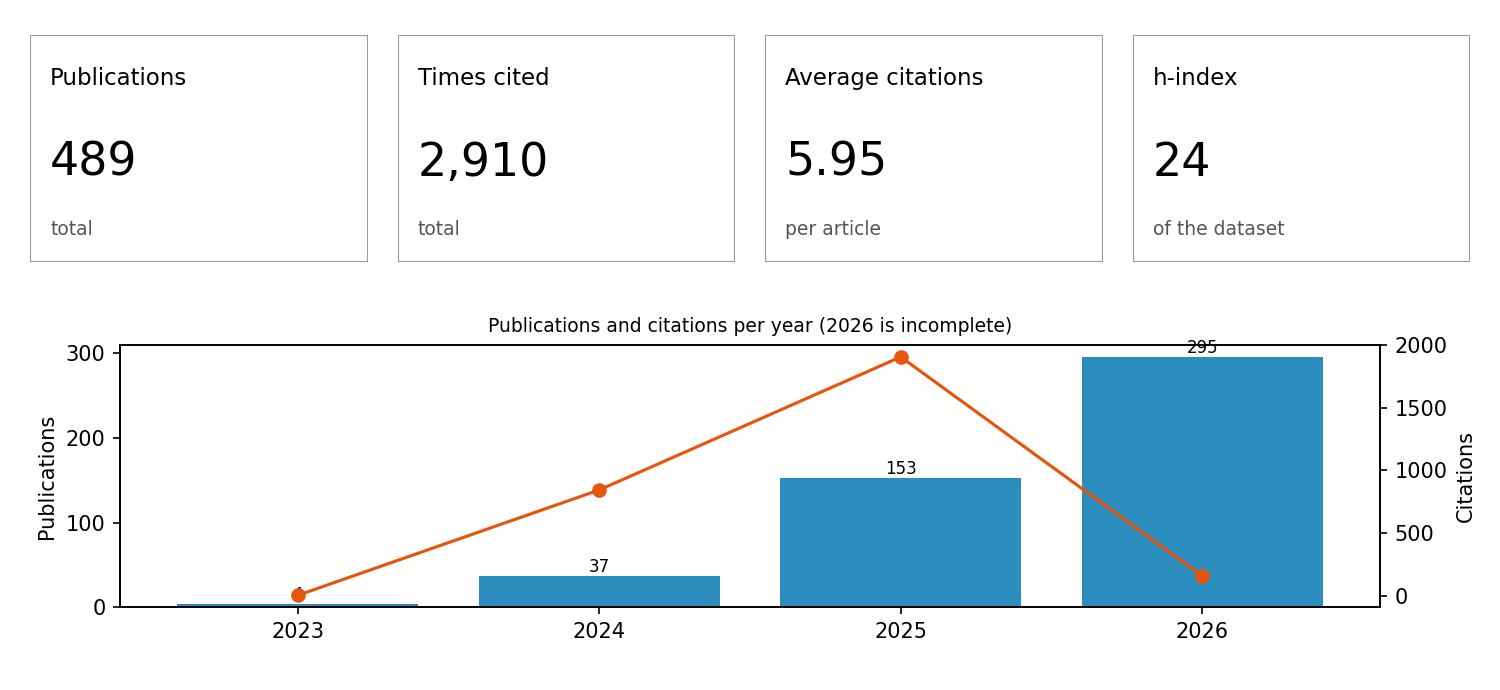
\includegraphics[width=\textwidth]{figures/gambar1_ringkasan.png}
\par\vspace{2pt}Source: Authors' analysis of OpenAlex data.
\caption{Summary of publications and citations in the dataset}
\label{fig:summary}
\end{figure}

\subsection{Citation Analysis}
The ten most cited documents all concern LLMs at the edge or small language models (Table~\ref{tab:A}). None addresses inventory or business operations.

\begin{table}[htbp]
\centering
\small
\caption{Top 10 document citation analysis}
\label{tab:A}
\begin{tabularx}{\textwidth}{|c|l|Y|c|}
\hline
\textbf{Rank} & \textbf{Author} & \textbf{Title} & \textbf{Citation} \\ \hline
1 & Ji Lin et al. & AWQ: Activation-aware Weight Quantization for On-Device LLM Compression and Acceleration & 273 \\ \hline
2 & Guanqiao Qu et al. & Mobile Edge Intelligence for Large Language Models: A Contemporary Survey & 240 \\ \hline
3 & Mingjin Zhang et al. & EdgeShard: Efficient LLM Inference via Collaborative Edge Computing & 227 \\ \hline
4 & Othmane Friha et al. & LLM-Based Edge Intelligence: A Comprehensive Survey on Architectures, Applications, Security... & 194 \\ \hline
5 & Yue Zheng et al. & A Review on Edge Large Language Models: Design, Execution, and Applications & 168 \\ \hline
6 & Fali Wang et al. & A Comprehensive Survey of Small Language Models in the Era of Large Language Models:... & 105 \\ \hline
7 & Zheng Lin et al. & Pushing Large Language Models to the 6G Edge: Vision, Challenges, and Opportunities & 92 \\ \hline
8 & Xinyuan Zhang et al. & Beyond the Cloud: Edge Inference for Generative Large Language Models in Wireless Networks & 77 \\ \hline
9 & Kailai Sun et al. & A review of AI edge devices and lightweight CNN and LLM deployment & 72 \\ \hline
10 & Rongjie Yi et al. & EdgeMoE: Empowering Sparse Large Language Models on Mobile Devices & 68 \\ \hline
\end{tabularx}
\par\vspace{2pt}{\normalsize Source: Authors' analysis of OpenAlex data.}
\end{table}


Authors and sources were counted by OpenAlex identifiers. The 489 articles carry 1{,}687 distinct author identifiers but 1{,}812 distinct author names, so counting names would have overstated the number of authors by 125. The most productive authors have four or five articles each (Table~\ref{tab:H}), and only 12 authors have three or more, which means that no small group dominates the field. The articles appear in 321 distinct sources. The most frequent are \textit{IEEE Transactions on Mobile Computing} with 20 articles, \textit{IEEE Access} with 14, and \textit{IEEE Internet of Things Journal} with 10 (Table~\ref{tab:I}). Among institutions, Tsinghua University leads with 10 articles, followed by South China University of Technology with 9 and the Beijing University of Posts and Telecommunications and Nanyang Technological University with 8 each.

\begin{table}[htbp]
\centering
\small
\caption{Most productive authors, counted by OpenAlex author ID (so that name variants are not counted twice); citations are global OpenAlex counts of the authors' articles in the dataset.}
\label{tab:H}
\begin{tabularx}{\textwidth}{Ylrr}
\toprule
\textbf{Rank} & \textbf{Author (OpenAlex author ID)} & \textbf{Articles} & \textbf{Citations} \\
\midrule
1 & Dusit Tao Niyato & 5 & 136 \\
2 & Kaibin Huang & 4 & 334 \\
3 & Partha Pratim Ray & 4 & 4 \\
4 & Mohan P. Pradhan & 4 & 4 \\
5 & Xianhao Chen & 3 & 333 \\
6 & Jiannong Cao & 3 & 253 \\
7 & Mingjin Zhang & 3 & 238 \\
8 & Mangesh Pujari & 3 & 8 \\
9 & Anil Kumar Pakina & 3 & 8 \\
10 & Tinoosh Mohsenin & 3 & 7 \\
\bottomrule
\end{tabularx}
\end{table}

\begin{table}[htbp]
\centering
\small
\caption{Most frequent sources, counted by OpenAlex source ID.}
\label{tab:I}
\begin{tabularx}{\textwidth}{rYrr}
\toprule
\textbf{Rank} & \textbf{Source (OpenAlex source ID)} & \textbf{Articles} & \textbf{Citations} \\
\midrule
1 & IEEE Transactions on Mobile Computing & 20 & 159 \\
2 & IEEE Access & 14 & 73 \\
3 & IEEE Internet of Things Journal & 10 & 264 \\
4 & Electronics & 7 & 28 \\
5 & Applied Sciences & 7 & 2 \\
6 & INTERANTIONAL JOURNAL OF SCIENTIFIC RESEARCH IN ENGINEERING AND MANAGEMENT & 7 & 0 \\
7 & Expert Systems with Applications & 5 & 2 \\
8 & International Journal for Research in Applied Science and Engineering Technology & 5 & 0 \\
9 & IEEE Network & 4 & 84 \\
10 & Scientific Reports & 4 & 23 \\
\bottomrule
\end{tabularx}
\end{table}


Country data are missing for 117 articles (24\%). In the rest, China contributes 113 articles, the United States 89, India 43, South Korea 31, and Hong Kong 28. Collaboration across borders is limited: only 86 articles (18\%) have authors from two or more countries. The most frequent pairs are Hong Kong and China (15 articles), the United States and China (11), and China and Singapore (9).

\subsection{Co-citation Analysis}
The articles cite 7{,}357 distinct references. Of these, 347 are cited by at least three articles of the dataset once ten data artefacts are removed (Section~3.4), and they form four clusters of 127, 95, 66, and 59 references (Table~\ref{tab:E}, Figure~\ref{fig:cocit}). The author named the clusters after reading the titles of their most co-cited references. The most strongly linked references (Table~\ref{tab:D}) are foundations of efficient LLM inference: LLaMA, structured pruning, quantisation, memory management for model serving, and GPT-3.

\begin{table}[htbp]
\centering
\small
\caption{Top 10 documents by co-citation total link strength (TLS); citations are counted within the dataset.}
\label{tab:D}
\begin{tabularx}{\textwidth}{rYrrr}
\toprule
\textbf{Rank} & \textbf{Document} & \textbf{Citations (within dataset)} & \textbf{TLS} & \textbf{Cluster} \\
\midrule
1 & Touvron (2023), LLaMA: Open and Efficient Foundation Language Models & 13 & 391 & 2 \\
2 & Ma (2023), LLM-Pruner: On the Structural Pruning of Large Language Models & 15 & 386 & 2 \\
3 & Shen (2024), Agile-Quant: Activation-Guided Quantization for Faster Inference of LLMs on the... & 10 & 379 & 3 \\
4 & Kwon (2023), Efficient Memory Management for Large Language Model Serving with PagedAttention & 19 & 369 & 2 \\
5 & B. (2020), Language Models are Few-Shot Learners & 16 & 358 & 2 \\
6 & Liu (2024), LLM-QAT: Data-Free Quantization Aware Training for Large Language Models & 10 & 332 & 2 \\
7 & Dettmers (2023), QLoRA: Efficient Finetuning of Quantized LLMs & 20 & 306 & 2 \\
8 & Alizadeh (2024), LLM in a flash: Efficient Large Language Model Inference with Limited Memory & 12 & 299 & 3 \\
9 & Vaswani (2025), Attention Is All You Need & 12 & 295 & 2 \\
10 & Ainslie (2023), GQA: Training Generalized Multi-Query Transformer Models from Multi-Head... & 9 & 295 & 2 \\
\bottomrule
\end{tabularx}
\end{table}


\begin{figure}[htbp]
\centering
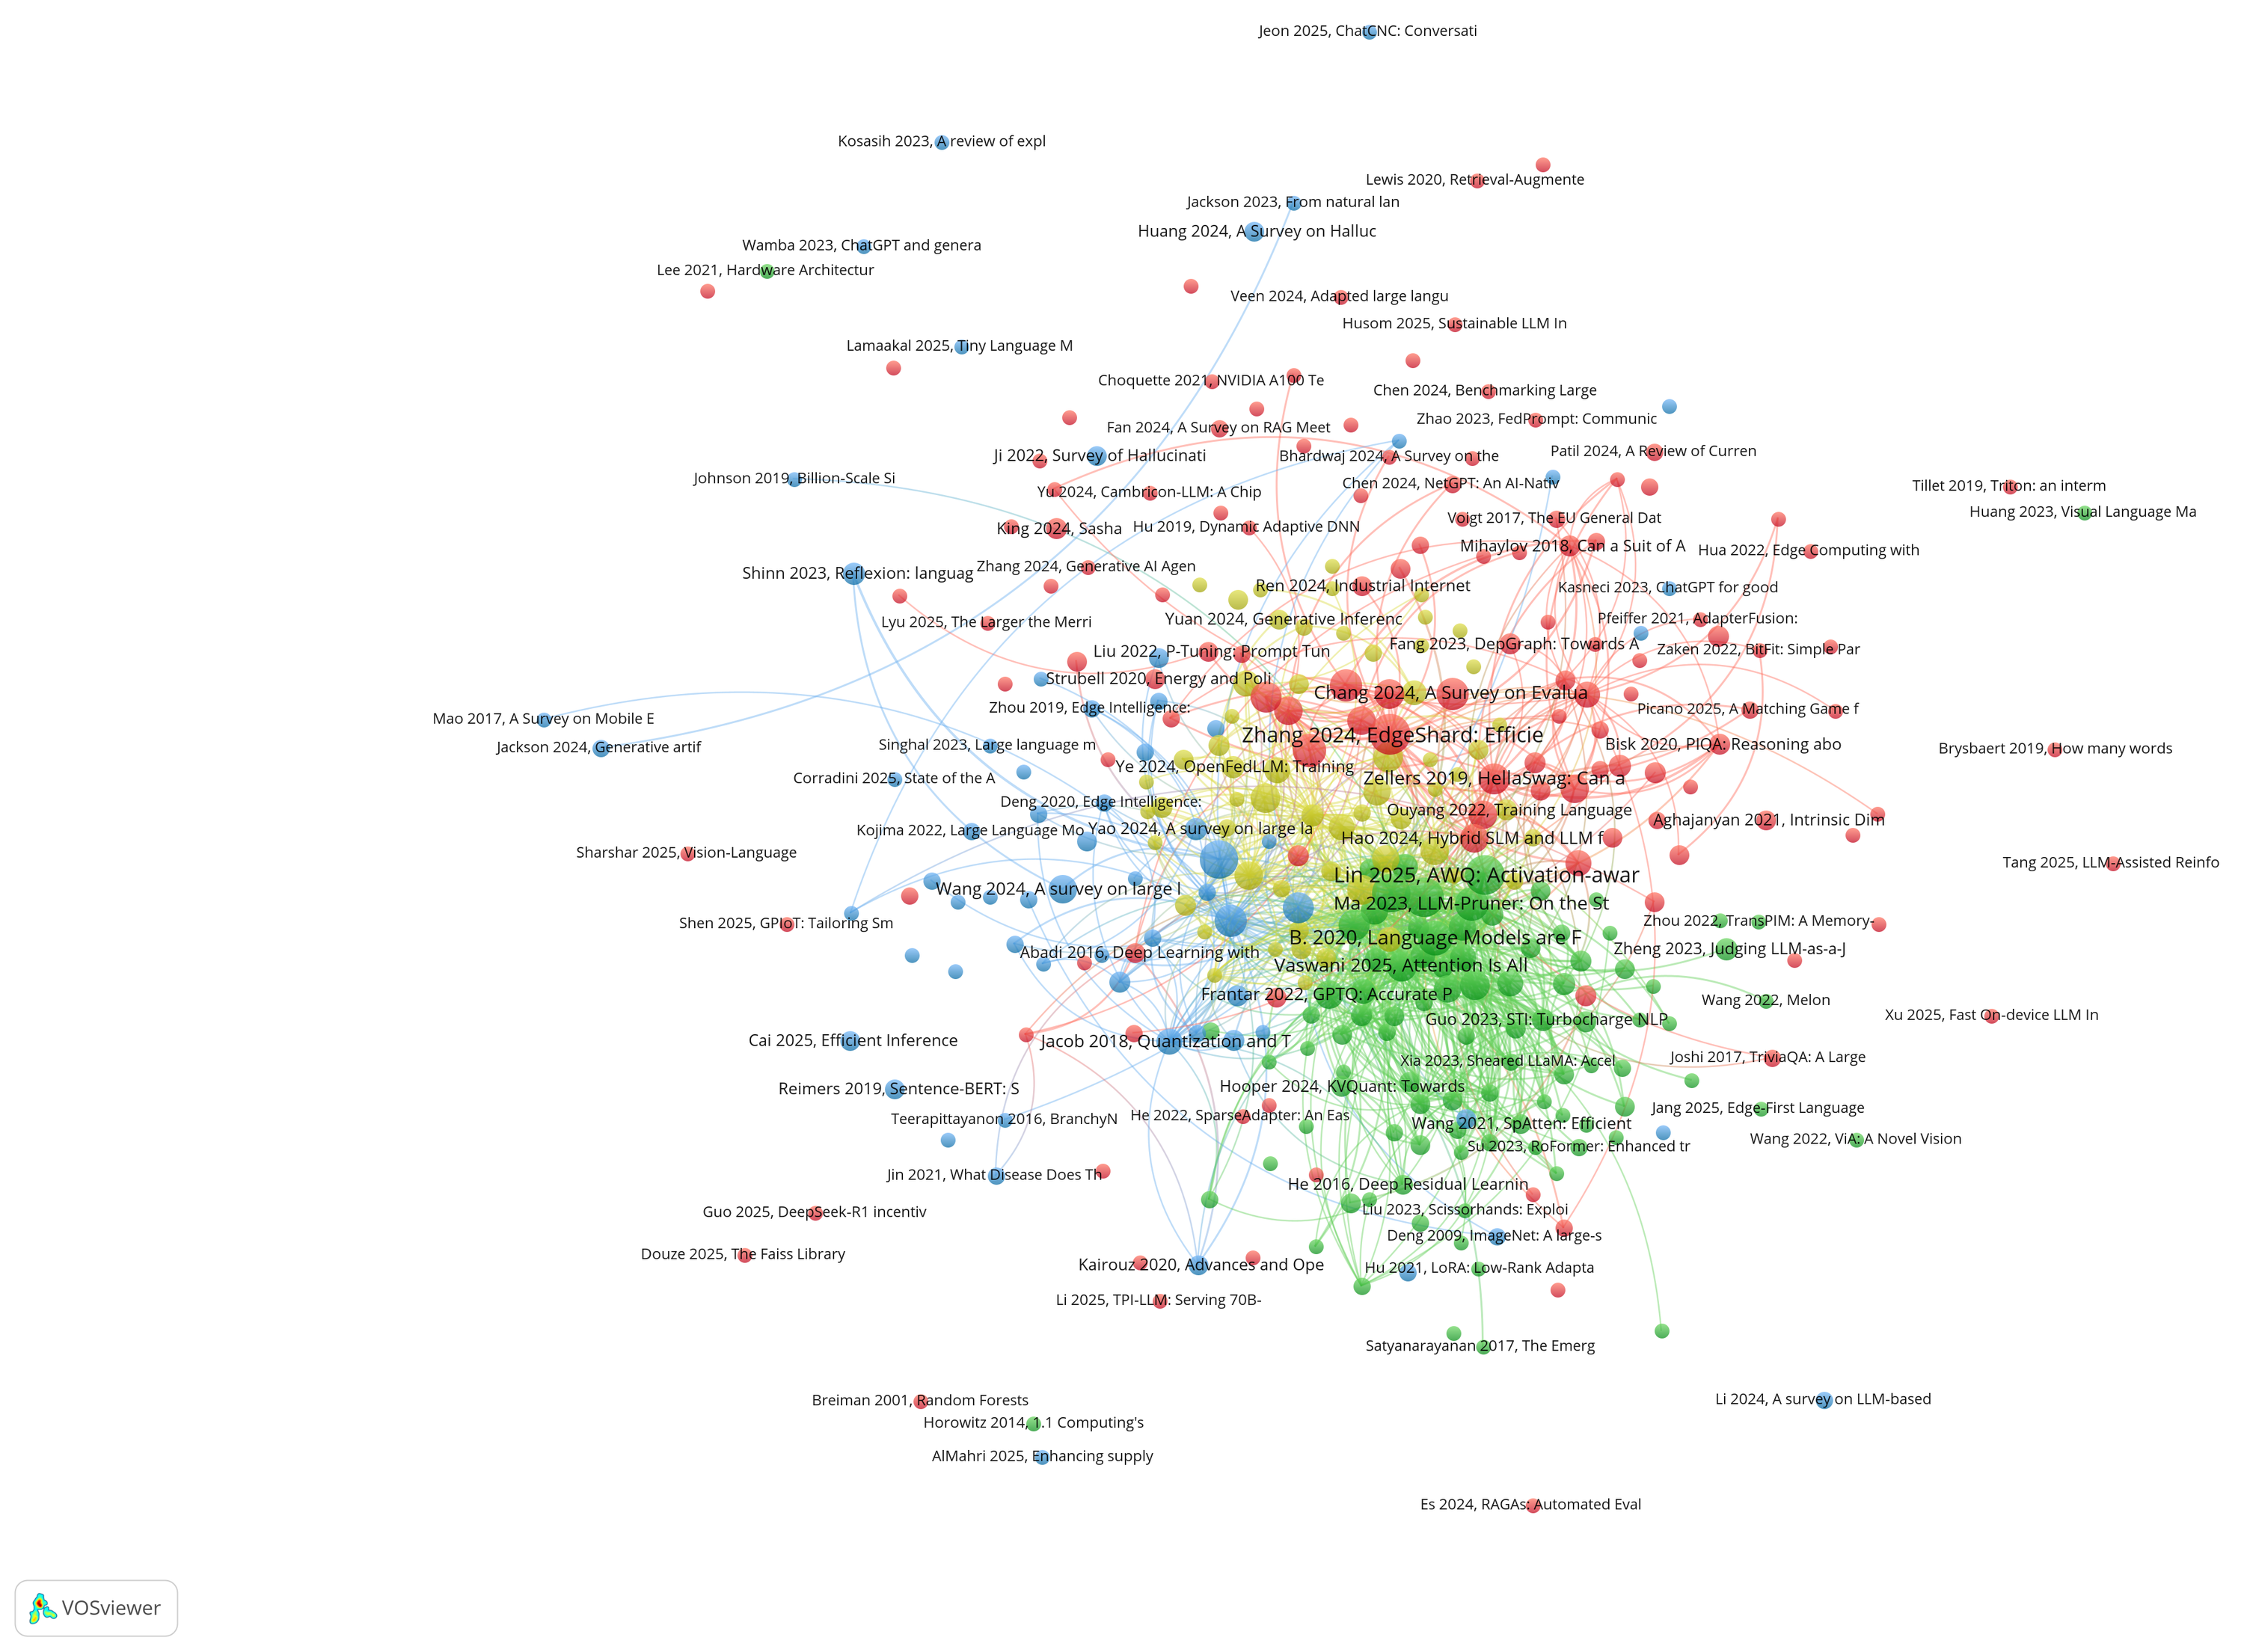
\includegraphics[width=\textwidth]{figures/vos_cocitation.png}
\par\vspace{2pt}Source: Author interpretation based on VOSviewer analysis.
\caption{Co-citation analysis of LLM research (347 references; colours show the four clusters; VOSviewer chooses which labels to show)}
\label{fig:cocit}
\end{figure}

The first cluster (red), collaborative edge--cloud LLM serving and its evaluation, joins serving systems and surveys with the benchmarks used to evaluate them. Its most co-cited references are EdgeShard and surveys of edge and mobile-edge LLMs, alongside standard benchmarks (HellaSwag, WinoGrande, GLUE, PIQA) and work on prompt tuning and federated fine-tuning. The second cluster (green), model compression and efficient inference foundations, is dominated by efficiency methods, namely QLoRA, AWQ, PagedAttention, LLM-Pruner, PowerInfer, GPTQ, and FlashAttention, with foundation papers such as GPT-3 and LLaMA as a smaller layer.

The third (blue) and fourth (yellow) clusters are heterogeneous. The blue cluster, shared foundations of reasoning, agents, and supply chain AI, combines chain-of-thought prompting, BERT, edge computing visions, quantisation basics, and federated learning with the only agent-related references, a survey of LLM-based autonomous agents and Reflexion. It also holds the six references on generative AI in supply chain and operations management: Jackson (2024), Wamba (2023), Jackson (2023), Kosasih (2023), AlMahri (2025), and a study of machine monitoring with LLMs (Jeon, 2025). \todo{read and verify these references before interpreting them} The yellow cluster, mobile inference and decentralised adaptation, mixes inference under memory limits, parameter-efficient and federated tuning, the Transformers library, early sequence models, and a few application studies, for example on LLMs in medicine and cyber threat detection. Both names describe the main strand rather than every member, and both clusters are better read as background than as topics.

\begin{table}[htbp]
\centering
\footnotesize
\caption{Co-citation clusters on LLM research}
\label{tab:E}
\begin{tabularx}{\textwidth}{|l|Y|c|Y|}
\hline
\textbf{Cluster No and colour} & \textbf{Cluster label} & \textbf{Number of articles} & \textbf{Representative publication} \\ \hline
1 (red) & Edge LLM surveys, collaborative serving, and NLP benchmarks & 128 & Zhang (2024), EdgeShard: Efficient LLM Inference via Collaborative Edge Computing \\ \hline
2 (green) & Quantisation, pruning, and serving efficiency, with foundation models & 95 & Dettmers (2023), QLoRA: Efficient Finetuning of Quantized LLMs \\ \hline
3 (blue) & Mixed background: efficient inference, federated and parameter-efficient tuning, early applications & 58 & Alizadeh (2024), LLM in a flash: Efficient Large Language Model Inference with Limited Memory \\ \hline
4 (yellow) & General background: reasoning, edge computing visions, LLM agents, compression basics & 57 & Wei (2022), Chain-Of-Thought Prompting Elicits Reasoning in Large Language Models \\ \hline
5 (purple) & Generative AI in supply chain and operations management & 6 & Jackson (2024), Generative artificial intelligence in supply chain and operations management: a... \\ \hline
\end{tabularx}
\par\vspace{2pt}{\normalsize Source: Author interpretation based on VOSviewer analysis.}
\end{table}


The overall partition is not stable. With the 485 articles screened before the third pass, the same threshold gave five clusters, the fifth consisting of the six supply chain references, and removing two further suspect references had changed that result from four clusters to five. Across 21 repeated runs on the present data (20 seeds and a greedy algorithm), the number of clusters ranged from three to five. The network is also very dense, with about 14{,}000 links among 347 references, because an article with a long reference list creates many pairs at once. The exact composition of the large clusters should therefore not be relied on. One feature is more robust. Of four references on generative AI and AI in supply chains (Jackson 2024, Wamba 2023, AlMahri 2025, and Kosasih 2023), at least three sat in the same small cluster of 4 to 13 references in 14 of the 21 runs; in the other seven runs, as in the map reported here, they were absorbed into a larger mixed cluster of 60 to 160 references. The data thus support a modest conclusion: references on generative AI in supply chains are co-cited mainly with each other and with general background work, and rarely with the efficient-inference literature. The business stream has no broad shared foundation yet, and it is a very small group.

\subsection{Co-word Analysis}
Of 2{,}142 distinct keywords, 69 occur at least eight times, and they form three clusters of 24, 23, and 22 keywords (Tables~\ref{tab:F} and \ref{tab:G}, Figure~\ref{fig:coword}). The author named the clusters after reading their keywords and the ten most representative articles of each.

\begin{table}[htbp]
\centering
\small
\caption{Top 15 keywords in the co-occurrence of keywords analysis}
\label{tab:F}
\begin{tabularx}{\textwidth}{|c|Y|c|c|}
\hline
\textbf{Rank} & \textbf{Keyword} & \textbf{Occurrences} & \textbf{Total link strength} \\ \hline
1 & edge computing & 86 & 237 \\ \hline
2 & on-device inference & 55 & 136 \\ \hline
3 & small language models & 55 & 151 \\ \hline
4 & edge deployment & 51 & 127 \\ \hline
5 & model compression & 51 & 193 \\ \hline
6 & retrieval-augmented generation & 47 & 109 \\ \hline
7 & edge devices & 40 & 84 \\ \hline
8 & energy efficiency & 38 & 125 \\ \hline
9 & resource-constrained devices & 37 & 132 \\ \hline
10 & multi-agent systems & 36 & 73 \\ \hline
11 & agentic ai & 26 & 61 \\ \hline
12 & inference latency & 26 & 74 \\ \hline
13 & data privacy & 24 & 71 \\ \hline
14 & federated learning & 24 & 85 \\ \hline
15 & llm agents & 24 & 34 \\ \hline
\end{tabularx}
\par\vspace{2pt}{\normalsize Source: Author interpretation based on VOSviewer analysis.}
\end{table}


\begin{figure}[htbp]
\centering
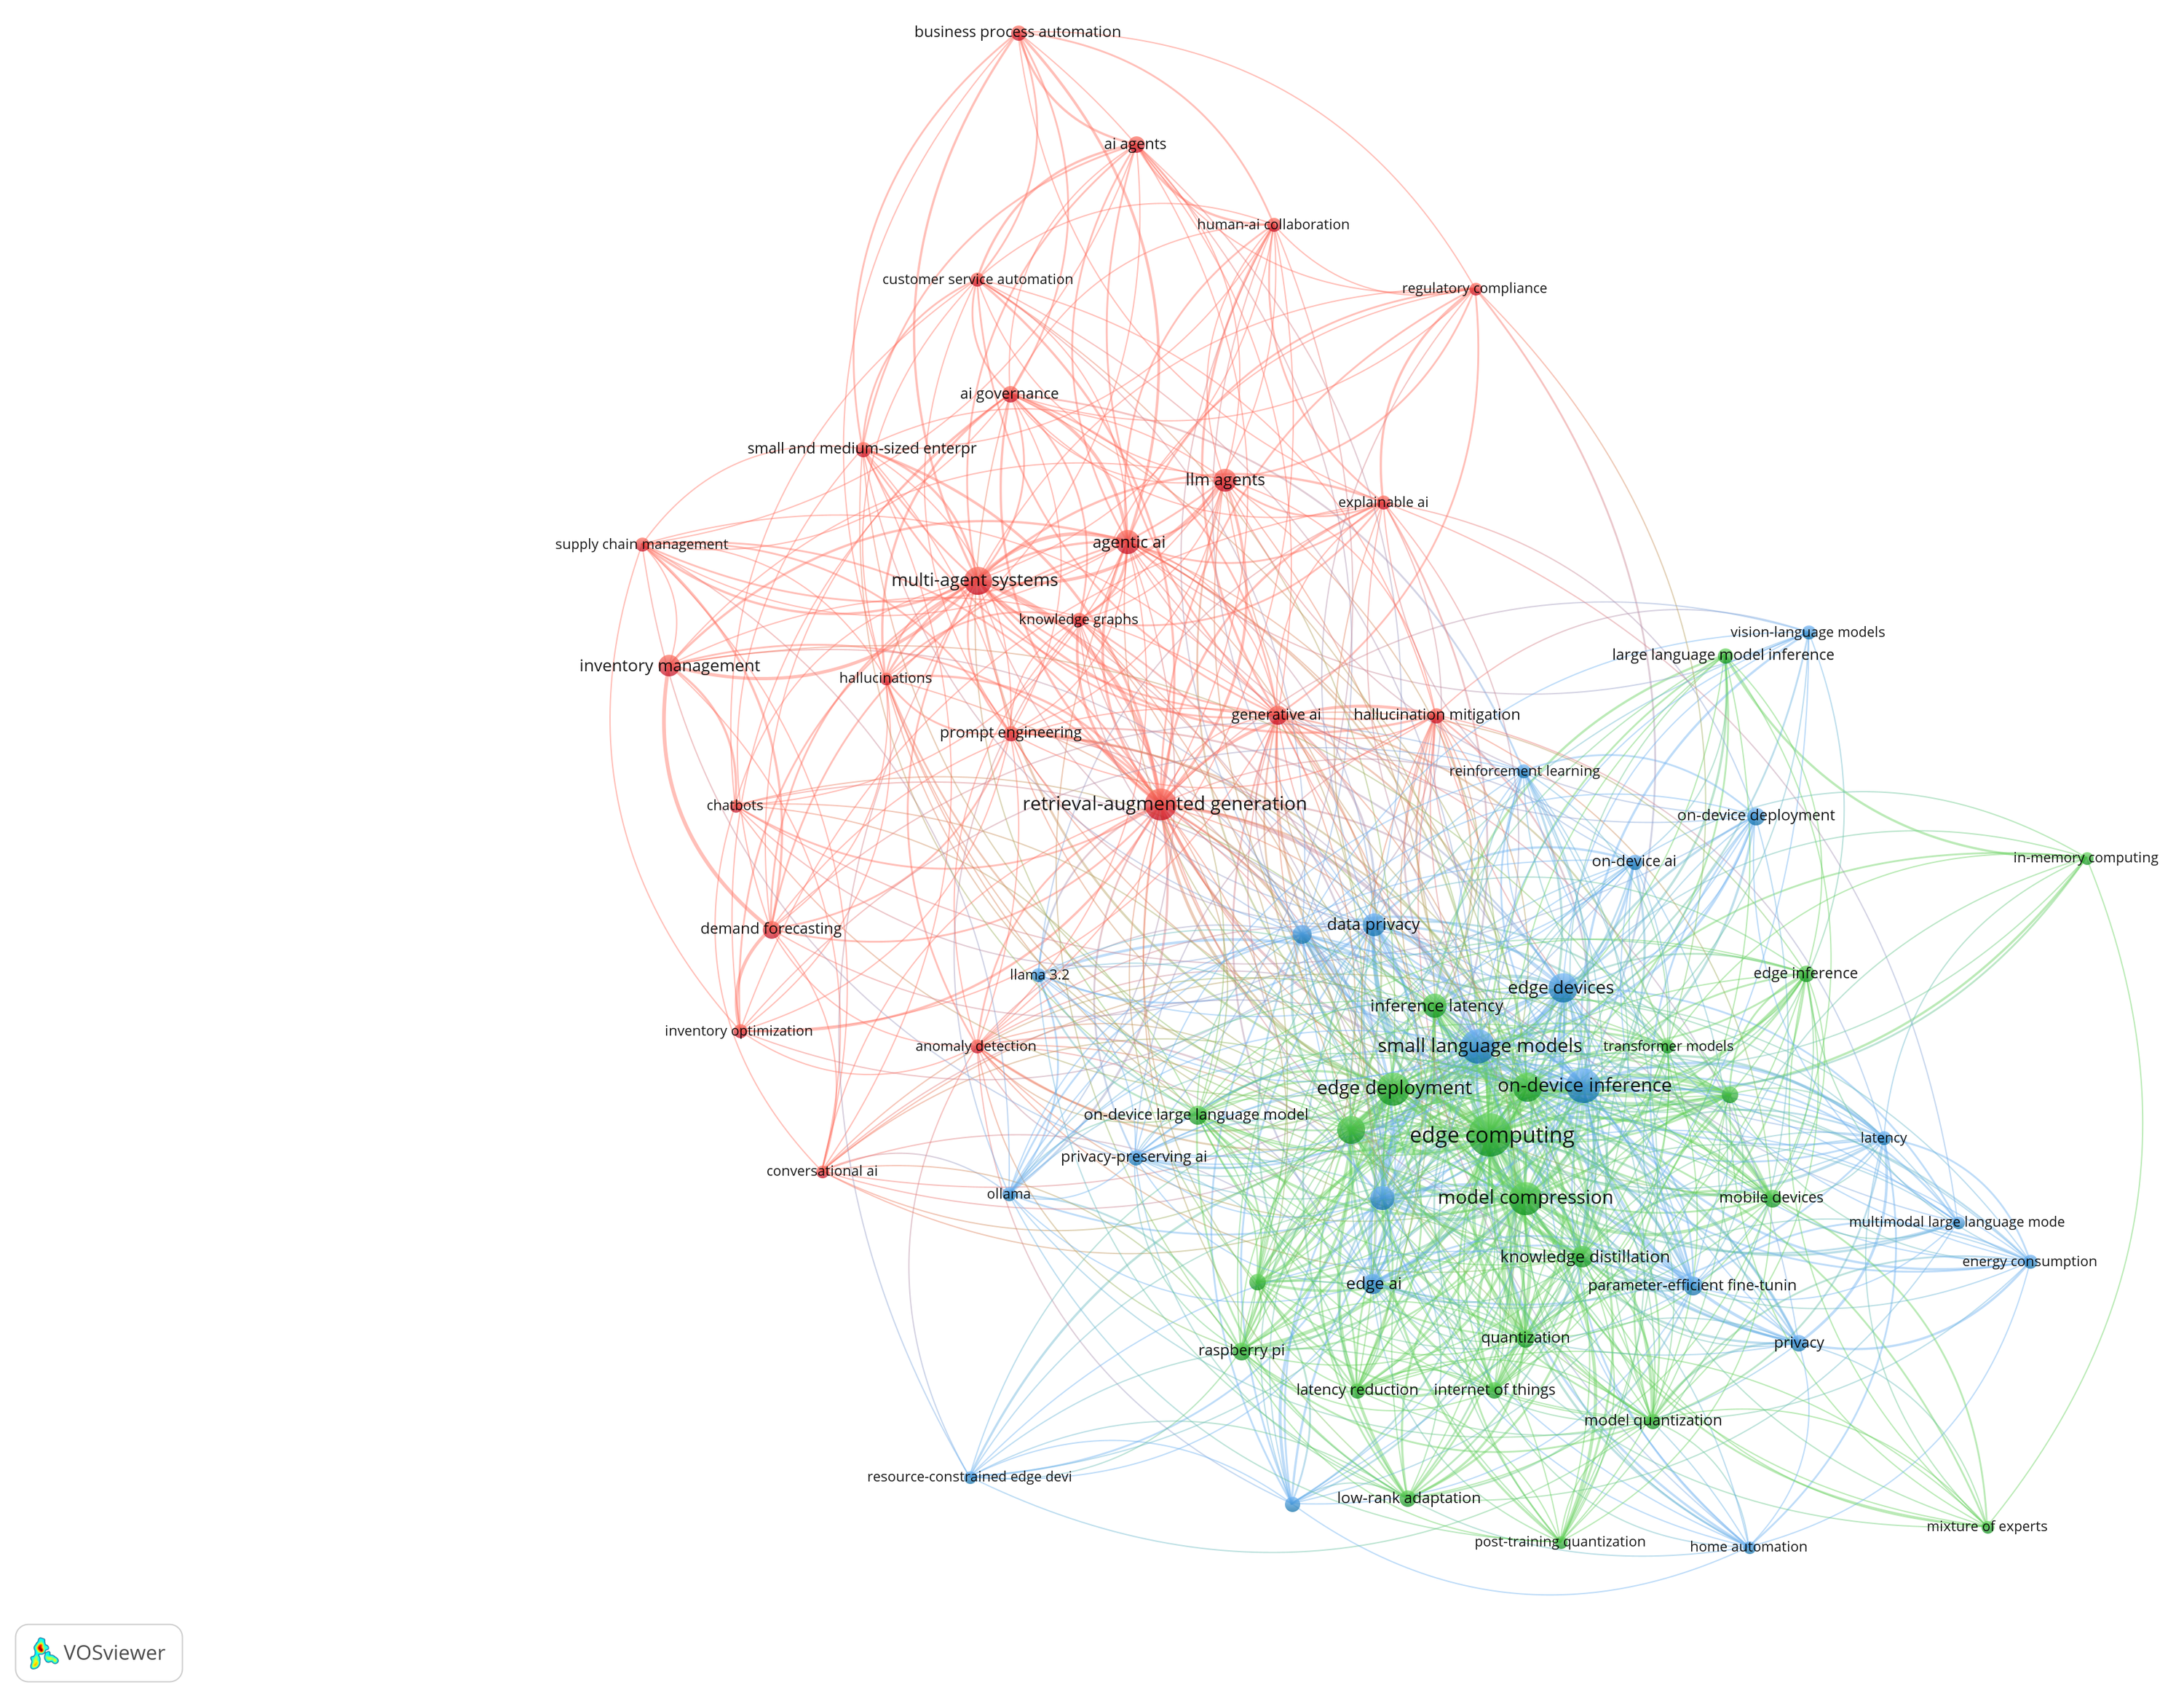
\includegraphics[width=\textwidth]{figures/vos_coword.png}
\par\vspace{2pt}Source: Author interpretation based on VOSviewer analysis.
\caption{Co-word analysis of LLM research (69 keywords with at least eight occurrences; node size is the number of articles; red: cluster 1, green: cluster 2, blue: cluster 3)}
\label{fig:coword}
\end{figure}

The red cluster, agentic and retrieval-augmented LLMs for business operations, centres on agents and retrieval-augmented generation in enterprise settings. It groups retrieval-augmented generation, multi-agent systems, agentic AI, and LLM agents with applications such as customer service, database querying, and business process automation. Inventory management and demand forecasting form a smaller strand within it. The green cluster concerns model compression and optimisation for edge deployment. Its articles are mostly surveys and frameworks about running LLMs under resource limits, and its keywords include model compression, energy efficiency, inference latency, knowledge distillation, and quantisation. The blue cluster concerns small language models and privacy-preserving on-device AI and has two strands, small models on the device and federated learning with differential privacy. It overlaps strongly with the green cluster, so the two differ mainly in emphasis.

\begin{table}[htbp]
\centering
\footnotesize
\caption{Co-word analysis on LLM research}
\label{tab:G}
\begin{tabularx}{\textwidth}{|l|Y|c|Y|}
\hline
\textbf{Cluster No and colour} & \textbf{Cluster label} & \textbf{Number of keywords} & \textbf{Representative keywords} \\ \hline
1 (red) & Agentic AI and RAG for enterprise applications (with an inventory sub-theme) & 24 & retrieval-augmented generation, multi-agent systems, agentic ai, llm agents, inventory management, generative ai, demand forecasting, ai agents \\ \hline
2 (green) & Compression and optimisation for edge LLM deployment & 23 & edge computing, model compression, edge deployment, energy efficiency, resource-constrained devices, inference latency, knowledge distillation, on-device large language models \\ \hline
3 (blue) & Small language models and privacy-preserving on-device learning & 21 & on-device inference, small language models, edge devices, federated learning, data privacy, edge ai, parameter-efficient fine-tuning, privacy preservation \\ \hline
\end{tabularx}
\par\vspace{2pt}{\normalsize Source: Author interpretation based on VOSviewer analysis.}
\end{table}


In 62 of 63 robustness runs, the agent and business keywords stayed in a cluster separate from the edge keywords; the exception was one seed at five occurrences, which produced four clusters. The runs varied the minimum occurrences (5, 8, and 12), used 20 random seeds, and included a greedy algorithm. Modularity was low, however, between 0.18 and 0.26, and between 19\% and 54\% of the link weight crossed cluster boundaries. The clusters are best described as loosely separated groups with limited links, not as disconnected fields.

\subsection{Bibliographic Coupling}
Of the 489 articles, 282 have reference data, and 184 of these share at least two references with another article. Without a citation threshold they form 12 clusters of 55, 38, 38, 18, 14, 5, 5, 3, 2, 2, 2, and 2 articles, of which seven have fewer than six articles. To obtain three to five clusters of at least six articles, as the supervisor's rule requires, only articles cited at least three times were kept. This left 72 articles in five clusters of 20, 20, 17, 13, and 2 articles, and the cluster of two was removed. The map thus shows 70 articles in four clusters. No other citation threshold between 0 and 20 met the rule, and with the 485 articles screened before the third pass, raising the minimum number of shared references to five or lowering the resolution of the algorithm did not meet it either. Table~\ref{tab:B} lists the ten articles with the highest total link strength, mostly surveys and system papers on edge LLMs, and Table~\ref{tab:C} summarises the four clusters. The author named the clusters after reading the titles of their articles. The names rest on titles only and are therefore weaker than those of the other two maps.

\begin{table}[htbp]
\centering
\small
\caption{Top 10 documents in the bibliographic coupling analysis}
\label{tab:B}
\begin{tabularx}{\textwidth}{cYcc}
\hline
\textbf{Rank} & \textbf{Publication} & \textbf{Citation} & \textbf{Total link strength} \\ \hline
1 & Wang et al. (2025), Empowering large language models to edge intelligence: A survey of edge... & 47 & 297 \\
2 & Friha et al. (2024), LLM-Based Edge Intelligence: A Comprehensive Survey on Architectures,... & 194 & 239 \\
3 & Piccialli et al. (2024), Federated and edge learning for large language models & 44 & 235 \\
4 & Sun et al. (2024), A review of AI edge devices and lightweight CNN and LLM deployment & 72 & 176 \\
5 & Zheng et al. (2025), A Review on Edge Large Language Models: Design, Execution, and Applications & 168 & 175 \\
6 & Xu et al. (2024), EdgeLLM: Fast On-Device LLM Inference With Speculative Decoding & 50 & 104 \\
7 & Yi et al. (2025), EdgeMoE: Empowering Sparse Large Language Models on Mobile Devices & 68 & 104 \\
8 & Qu et al. (2025), Mobile Edge Intelligence for Large Language Models: A Contemporary Survey & 240 & 80 \\
9 & Wang et al. (2025), Split Learning Based Cloud-Edge-End Collaborative Model Training in... & 5 & 77 \\
10 & Semerikov et al. (2025), Edge intelligence unleashed: a survey on deploying large language models in... & 20 & 75 \\ \hline
\end{tabularx}
\par\vspace{2pt}{\normalsize Source: Author interpretation based on VOSviewer analysis.}
\end{table}


All four clusters concern LLMs at the edge and differ in emphasis: efficient on-device inference on mobile hardware (cluster 1), edge LLM surveys and distributed fine-tuning (cluster 2), applied edge intelligence across domains (cluster 3), and privacy-preserving and personalised LLMs for IoT (cluster 4). Their boundaries should not be over-interpreted. Compared with the 485 articles screened before the third pass, only one added article entered the map, yet most clusters exchanged members. The only three articles from the agent and inventory blocks fall into three different clusters: decentralised agents in cluster 1, a pharmaceutical supply chain application in cluster 3, and privacy in multi-agent systems in cluster 4.

\begin{table}[htbp]
\centering
\small
\caption{Summary of bibliographic coupling clusters (clusters with at least five documents).}
\label{tab:C}
\begin{tabularx}{\textwidth}{llrYY}
\toprule
\textbf{Cluster (colour)} & \textbf{Cluster label} & \textbf{No. of publications} & \textbf{Source block} & \textbf{Representative publications} \\
\midrule
1 (red) & \todo{to be labelled} & 43 & B: 39, A: 2, A+C: 1, C: 1 & Friha et al. (2024), LLM-Based Edge Intelligence: A Comprehensive Survey on Architectures,...; Piccialli et al. (2024), Federated and edge learning for large language models \\
2 (green) & \todo{to be labelled} & 38 & B: 37, C: 1 & Semerikov et al. (2025), Edge intelligence unleashed: a survey on deploying large language models in...; Jiang et al. (2026), Edge large language models: a comprehensive survey \\
3 (blue) & \todo{to be labelled} & 35 & B: 34, A: 1 & Wang et al. (2025), Empowering large language models to edge intelligence: A survey of edge...; Zheng et al. (2025), A Review on Edge Large Language Models: Design, Execution, and Applications \\
4 (yellow) & \todo{to be labelled} & 24 & B: 24 & Duan et al. (2026), SoK: Towards a user-centric, privacy-preserving, and reliable AI agent via...; Zhuang et al. (2026), Resource-Efficient LLM Customization on Mobile Devices Through Proxy Submodel... \\
5 (purple) & \todo{to be labelled} & 14 & B: 14 & Eccles et al. (2025), Mosaic: Composite projection pruning for resource-efficient LLMs; Luo et al. (2026), CALSI: Context-Aware Layer Skipping Inference for On-Device LLM Serving \\
6 (cyan) & \todo{to be labelled} & 8 & A: 4, B: 3, C: 1 & Bhattacharyya et al. (2026), The economics of accuracy for medical reasoning with large language models; Pacella et al. (2026), Governed Agentic Process Automation: A Floor-Safety Guarantee for... \\
7 (orange) & \todo{to be labelled} & 5 & B: 5 & Joshi et al. (2026), Securing the Cognitive Layer: A Survey on Security Threats, Defenses, and...; Jeong et al. (2025), On-Device Intent Reasoning for Smart Home Agents Via Ontology-Augmented sLLMs \\
8 (?) & \todo{to be labelled} & 5 & C: 3, A+C: 1, A: 1 & Nakhost et al. (2025), Full automation or just a copilot? A study of large language models on spare...; Hamdan et al. (2026), Evaluating large language models for complex supply chain optimisation: a focus... \\
\bottomrule
\end{tabularx}
\end{table}


The threshold has a cost for the business stream. Of the 22 agent and inventory articles among the 184 connected ones, only 3 remain, and the cluster on LLM agents for supply chain and demand forecasting (five articles in the unfiltered map) is no longer visible. The unfiltered clustering was repeated with 20 random seeds and a greedy algorithm. The number of clusters varied from 11 to 15, and between 41\% and 73\% of the 22 articles (median 73\%) fell in clusters where business-related articles formed the majority. The business stream is thus a small and partly stable feature of the unfiltered coupling network, not a robust cluster with fixed membership, and it does not meet the citation threshold in the map reported here.

\subsection{Sensitivity to a Wider Search}
To see whether the findings depend on how narrowly the business block was searched, the search was widened once and the analysis repeated. The widening added generative-AI and ChatGPT terms and a longer list of business terms (supply chain, order management, restaurant, food and beverage) to the inventory block, and the repeated run of the original strings also returned 35 articles that were not in the first download. This gave 172 records not screened before; 37 from the Zenodo repository and 8 duplicate titles were removed, and the remaining 127 were screened with the same criteria. The model kept 55 (54 from the inventory block and 1 from the agent block), rejected 57, and marked 15 as doubtful; the doubtful ones were left out. The 14 kept articles on which the model reported low confidence were judged again in the third pass (Section~3.3). Twelve were confirmed and two were rejected; the two are versions of one study that credits the inventory gains to predictive rather than generative AI. The check therefore added 53 articles, 52 from the inventory block and 1 from the agent block. The year 2022 and a wider agent block were not added: the original strings return no article for 2022, and in a sample of 20 titles, the wider agent terms retrieved mostly language-model security and general chatbot articles.

With 542 articles, the 489 of the main dataset and the 53 added, of which 301 have reference data (55.5\%), the results changed in three ways.
\begin{itemize}
  \item \textbf{Co-word.} Only two clusters appeared at every threshold from 5 to 15 occurrences. At 8 occurrences, the first cluster (45 keywords) joins edge computing, model compression, and small language models and privacy; the second (35 keywords) joins generative AI, retrieval-augmented generation, inventory management, multi-agent systems, and demand forecasting. The earlier three clusters therefore reduce to a split between the two streams, and the rule of three to five clusters is not met at any threshold.
  \item \textbf{Co-citation and coupling.} At the thresholds used for the main maps (three citations), co-citation gave five clusters (116, 97, 67, 62, and 23 references). The fifth gathers references on generative AI and ChatGPT in operations and supply chains, for example \textcite{wamba2023} and \textcite{jackson2024}, together with a survey of hallucination. Coupling gave five clusters of at least six articles (19, 18, 17, 16, and 11), and the second, with 18 articles, is mixed: 12 come from the agent and inventory blocks and 6 from the device block. Both maps meet the rule of three to five clusters, and in both the business stream forms a group of its own once the wider search adds more business articles.
  \item \textbf{Robustness.} In all 63 runs of the same robustness check, the agent and business keywords stayed apart from the edge keywords. In 62 of them all business keywords sat in one cluster. Modularity was between 0.32 and 0.37, and between 11.2\% and 18.3\% of the link weight crossed cluster boundaries, so the separation is stronger than in the main data (0.18 to 0.26 and 19\% to 54\%).
\end{itemize}
The separation of the business stream from the edge stream thus holds, and is clearer, with the wider search. What does not hold is the number and the boundaries of the clusters, which depend on the data and the thresholds. The maps and tables in this article therefore use the 489 articles of the main search, and the analysis for 542 articles is kept as a sensitivity check (files in \texttt{analysis/Hasil\_uji542}).

\subsection{Thematic Map and Emerging Topics}
Each co-word cluster was also placed on a centrality--density map (Figure~\ref{fig:tema}, Table~\ref{tab:L}). At the eight-occurrence threshold, the compression cluster has both high density and high centrality, which marks a well-developed central theme. The small-model and privacy cluster has high centrality but lower density, as a transversal basic theme would. The agent and business cluster has the lowest centrality (217) and a middling density, so it is the least connected to the rest of the field. At a threshold of five occurrences it has the second lowest centrality (349); only a small cluster of seven privacy and local-runtime keywords, among them Ollama, is less central (204). With only three clusters the picture is coarse, and the quadrant labels depend on the cut-off.

\begin{figure}[htbp]
\centering
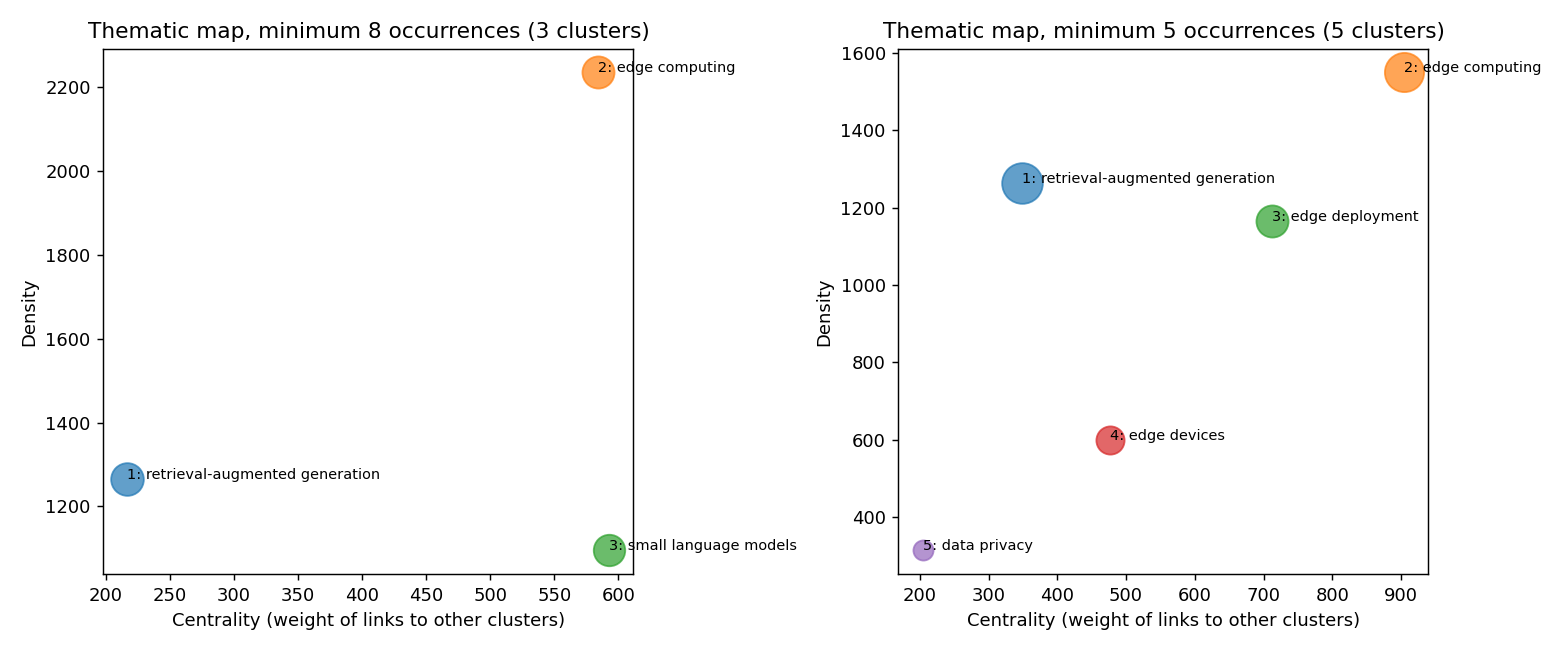
\includegraphics[width=\textwidth]{figures/peta_tema.png}
\par\vspace{2pt}Source: Authors' analysis of OpenAlex data.
\caption{Thematic maps from the co-word clusters (left: at least eight occurrences; right: at least five)}
\label{fig:tema}
\end{figure}
\begin{table}[htbp]
\centering
\small
\caption{Thematic map values for the three co-word clusters (minimum eight occurrences): centrality is the weight of links to other clusters; density is 100 times the internal link weight per keyword.}
\label{tab:L}
\begin{tabularx}{\textwidth}{rrrrY}
\toprule
\textbf{Cluster} & \textbf{Keywords} & \textbf{Centrality} & \textbf{Density} & \textbf{Leading keywords} \\
\midrule
1 & 24 & 213 & 1266.7 & retrieval-augmented generation, multi-agent systems, agentic ai, llm agents \\
2 & 23 & 579 & 2173.9 & edge computing, model compression, edge deployment, energy efficiency \\
3 & 21 & 574 & 1133.3 & small language models, on-device inference, edge devices, federated learning \\
\bottomrule
\end{tabularx}
\end{table}


Between 2025 and 2026 the share of articles carrying agent and retrieval keywords rises, while the share carrying generic edge keywords falls (Table~\ref{tab:K}). Retrieval-augmented generation grows from 4.6\% to 12.5\% of articles, small and medium-sized enterprises from 0\% to 4.1\%, multi-agent systems from 5.2\% to 8.8\%, and LLM agents from 2.6\% to 5.8\%. Resource-constrained devices fall from 13.1\% to 5.1\% and edge computing from 20.9\% to 15.9\%. Because 2026 is incomplete, this describes a change in composition, not in absolute numbers. Colouring keywords by mean publication year (Figure~\ref{fig:trendmap}) points the same way. Business-oriented keywords such as small and medium-sized enterprises (mean year 2026.0) and business process automation (2025.9) are newer than inventory management and demand forecasting, and local runtimes such as Ollama (2025.9) are newer than the Internet of Things (2024.9). The mean years span only about one year, so the result is best read as an early trend.

\begin{table}[htbp]
\centering
\small
\caption{Keywords with the largest falling (first five rows) and rising (last five rows) share of articles, 2025 (n = 153) and 2026 (n = 295)}
\label{tab:K}
\begin{tabularx}{\textwidth}{Yccccc}
\hline
\textbf{Keyword} & \textbf{Articles 2025} & \textbf{Articles 2026} & \textbf{Share 2025 (\%)} & \textbf{Share 2026 (\%)} & \textbf{Change (points)} \\ \hline
resource-constrained devices & 20 & 15 & 13.1 & 5.1 & -8.0 \\
edge computing & 32 & 47 & 20.9 & 15.9 & -5.0 \\
edge devices & 17 & 19 & 11.1 & 6.4 & -4.7 \\
internet of things & 8 & 2 & 5.2 & 0.7 & -4.6 \\
on-device inference & 20 & 29 & 13.1 & 9.8 & -3.2 \\
retrieval-augmented generation & 7 & 37 & 4.6 & 12.5 & 8.0 \\
small and medium-sized enterprises & 0 & 12 & 0.0 & 4.1 & 4.1 \\
multi-agent systems & 8 & 26 & 5.2 & 8.8 & 3.6 \\
hallucination mitigation & 1 & 11 & 0.7 & 3.7 & 3.1 \\
knowledge distillation & 4 & 17 & 2.6 & 5.8 & 3.1 \\ \hline
\end{tabularx}
\par\vspace{2pt}{\normalsize Source: Authors' analysis of OpenAlex data.}
\end{table}


\begin{figure}[htbp]
\centering
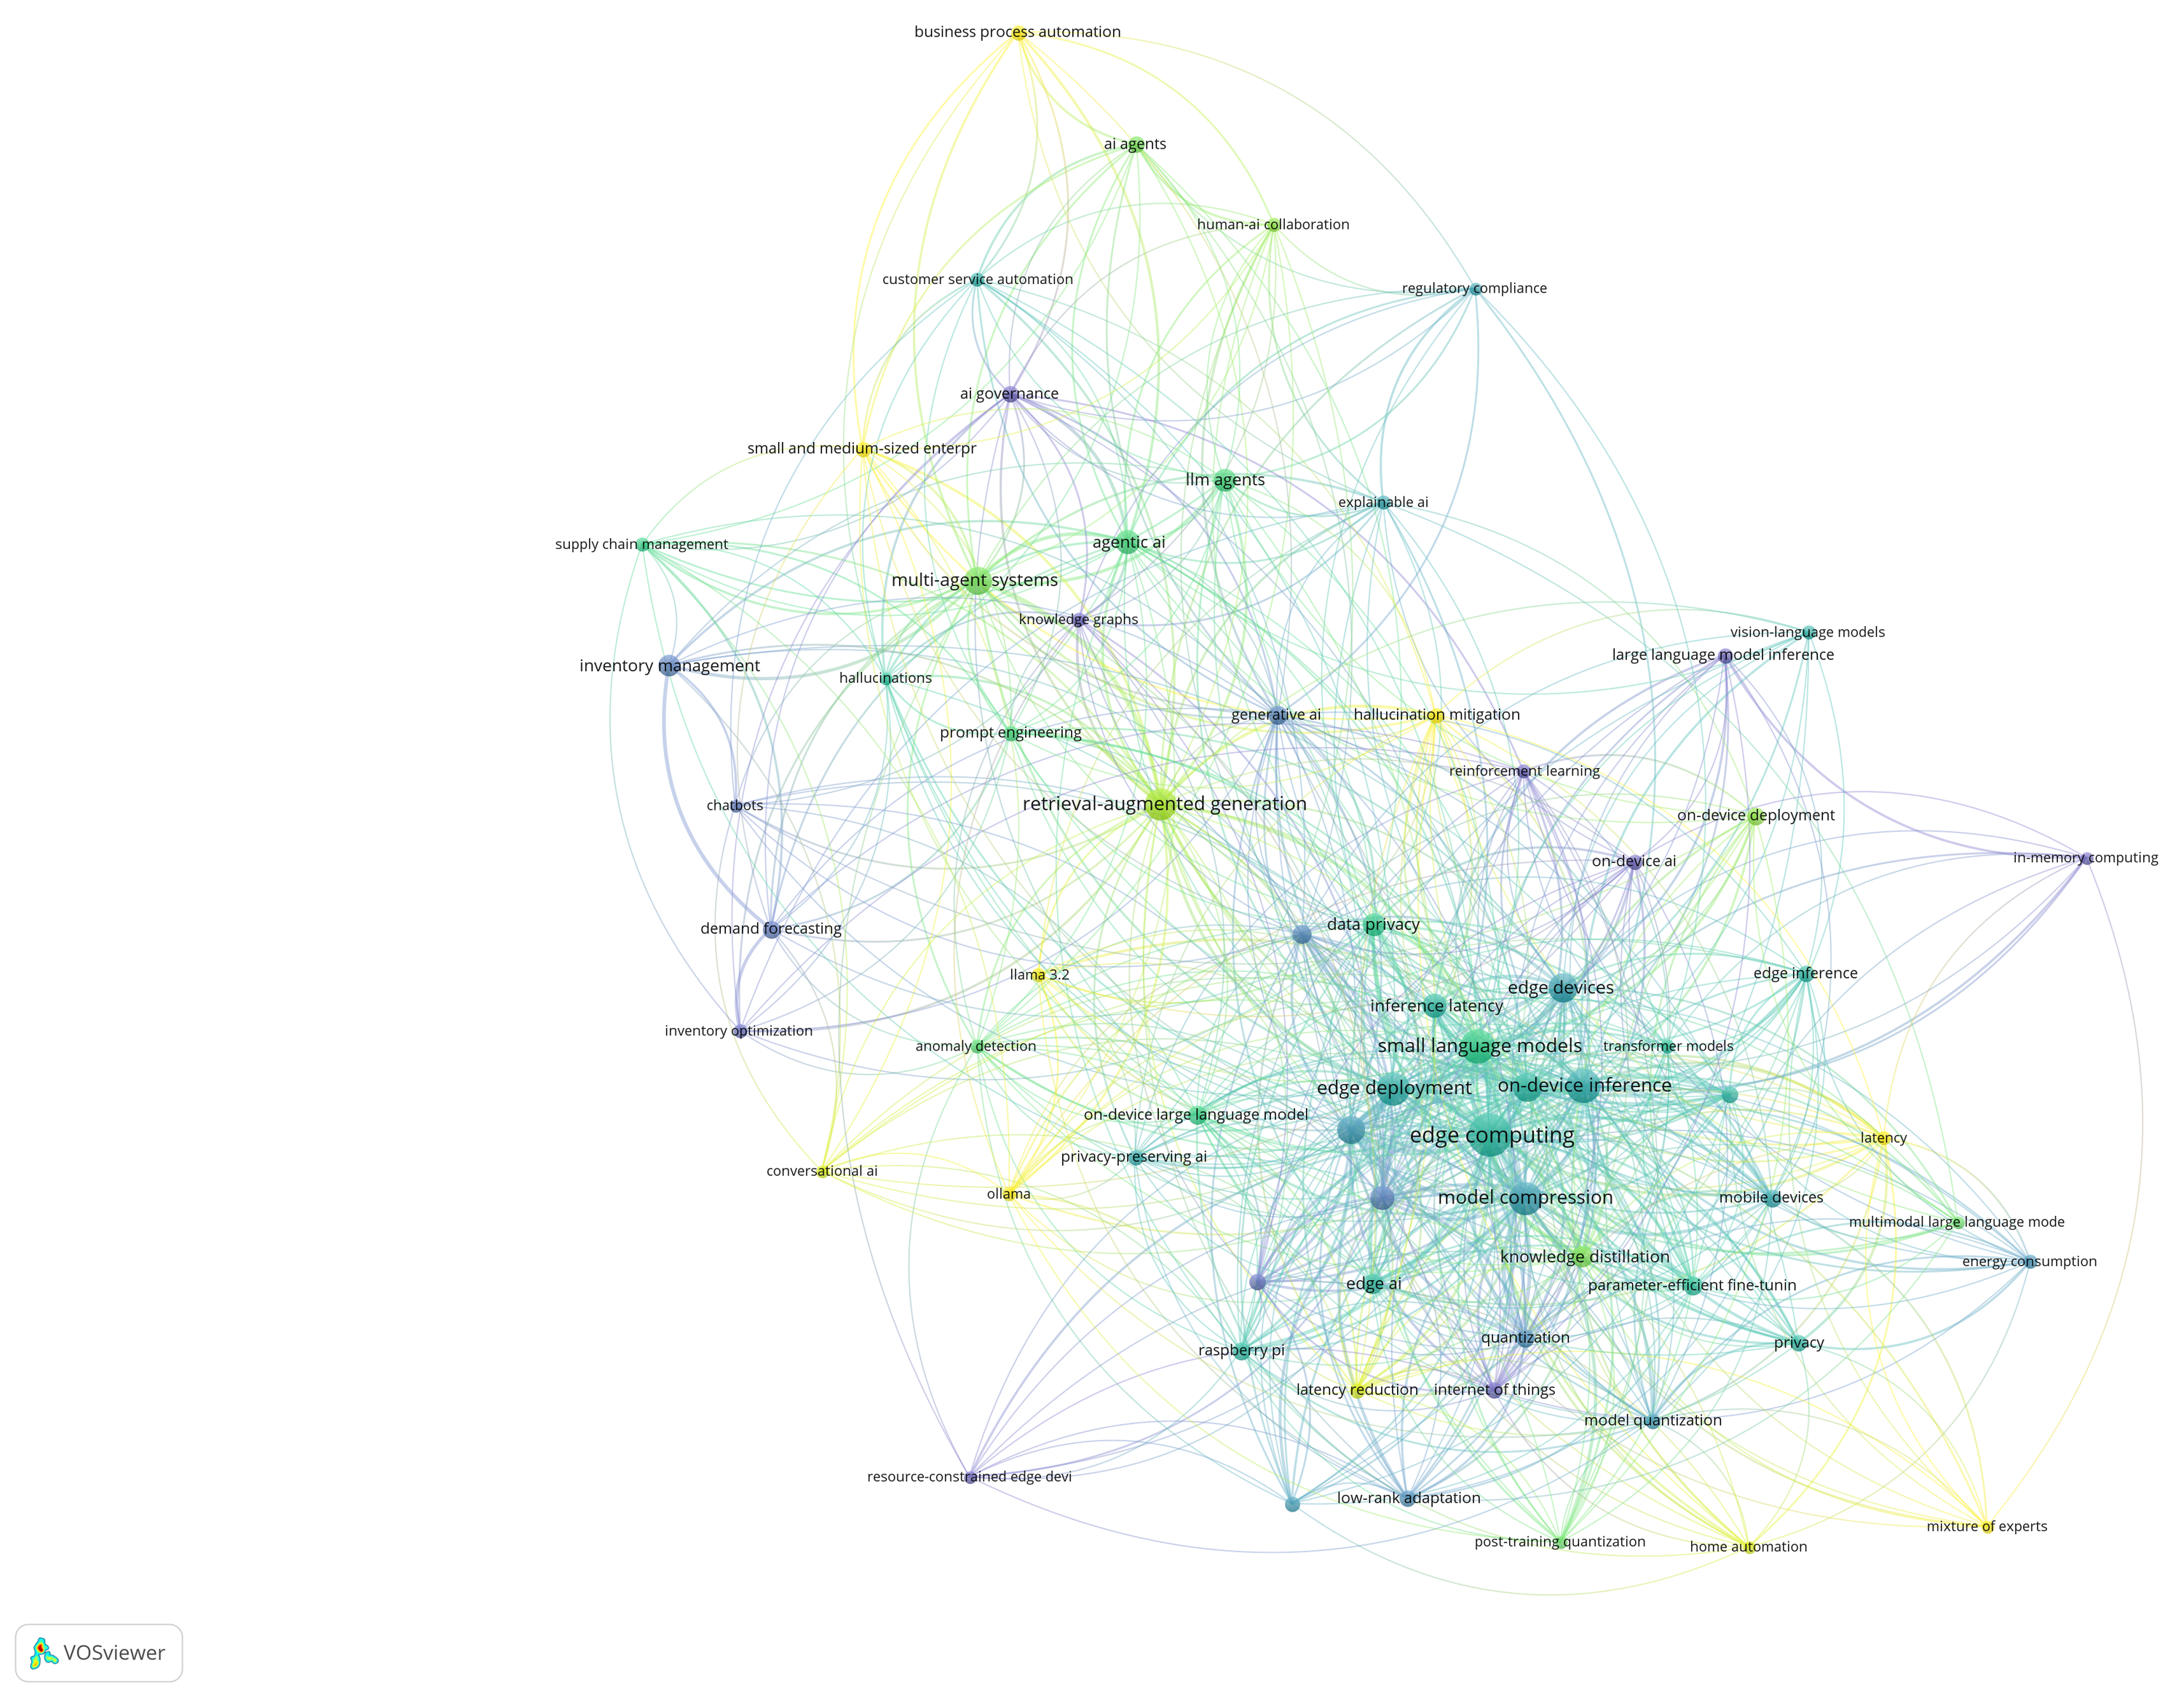
\includegraphics[width=\textwidth]{figures/vos_tren.png}
\par\vspace{2pt}Source: Author interpretation based on VOSviewer analysis.
\caption{Co-word overlay map coloured by mean publication year (purple: earlier, about 2024.9; yellow: more recent, about 2026.0)}
\label{fig:trendmap}
\end{figure}

\subsection{Sensitivity of the Search Strings}
The searches were repeated with five variations (Table~\ref{tab:J}). Every variation that only widened the strings retained all 489 articles of the final dataset. The title-only variant retained 61 (12\%), so searching abstracts is necessary. The searches were run with the 485 articles screened first; for the four articles added in the third pass, a later query showed that none has a title that matches the strings. Narrow changes, such as dropping the stock-market exclusion or adding inventory synonyms like SKU and stockout, altered the result by fewer than ten records. Widening the language-model terms (generative AI, GPT, ChatGPT, foundation models) or the device terms (TinyML, local LLM, smartphone, mobile device) added 512 and 576 records outside the cleaned baseline; part of each figure consists of the 93 baseline records removed as duplicates or Zenodo items. Eight added titles were read for each of the four widened variants. Most were marginal, for example generic generative AI in commerce or smartphone applications, but a few were relevant, such as work on offline document analysis with local language models. The core of the dataset is therefore stable, the boundary of the field is wide, and the baseline favours precision over recall. The added records were not screened, so their effect on the maps is unknown. \todo{screen the records added by V1 and V4 and repeat the co-word analysis}

\begin{table}[htbp]
\centering
\small
\caption{Sensitivity of the search strings. ``New'' counts records not in the cleaned baseline of 708 (it includes the 93 records that were removed as duplicates or Zenodo items in the baseline run).}
\label{tab:J}
\begin{tabularx}{\textwidth}{Yrlr}
\toprule
\textbf{Variant} & \textbf{Unique results} & \textbf{Final 485 retained} & \textbf{New outside the cleaned baseline} \\
\midrule
Baseline & 801 & 485 of 485 (100\%) & 93 \\
V1: broader LLM terms (+generative AI, GPT, ChatGPT, foundation model) & 1220 & 485 of 485 (100\%) & 512 \\
V2: block C without the stock-market exclusion & 810 & 485 of 485 (100\%) & 102 \\
V3: title only instead of title and abstract & 71 & 61 of 485 (13\%) & 8 \\
V4: broader device terms (+TinyML, local LLM, smartphone, mobile device) & 1284 & 485 of 485 (100\%) & 576 \\
V5: broader inventory terms (+SKU, stockout, warehouse management) & 808 & 485 of 485 (100\%) & 100 \\
\bottomrule
\end{tabularx}
\end{table}

